\documentclass[10pt,twocolumn,a4paper]{article}

% -------------------------------------------------
% Idioma y codificación
% -------------------------------------------------
\usepackage[T1]{fontenc}
\usepackage{lmodern}
\usepackage[english]{babel}

% -------------------------------------------------
% Formato del documento
% -------------------------------------------------
\usepackage[
    top=1.8cm,
    bottom=1.8cm,
    left=1.8cm,
    right=1.8cm,
    columnsep=0.7cm
]{geometry}

\usepackage{microtype}
\usepackage{parskip}

% -------------------------------------------------
% Matemáticas
% -------------------------------------------------
\usepackage{amsmath}
\usepackage{amssymb}
\usepackage{bm}

% -------------------------------------------------
% Figuras y tablas
% -------------------------------------------------
\usepackage{graphicx}
\usepackage{booktabs}
\usepackage{siunitx}

% -------------------------------------------------
% Enlaces y referencias
% -------------------------------------------------
\usepackage[hidelinks]{hyperref}

% Carpeta de imágenes
\graphicspath{{images/}}

% -------------------------------------------------
% Información del documento
% -------------------------------------------------
\title{
    \textbf{Multiple Goal Analysis\\
    Using Robot Heading}
}

\author{
    Julio Quejido Barrera\\
    Humanoide Robotik\\
    Julio's Laboratories
}

\date{\today}

% =================================================
\begin{document}
% =================================================

\maketitle

\begin{abstract}
This project extends the single-goal geometric analysis 
introduced in Project 1 to an environment containing 
multiple candidate goals. A robot heading vector is 
introduced to represent the direction in which the 
robot is facing. For each candidate goal, the scalar 
product between the robot heading and the normalized 
direction toward the goal is computed. This value 
is interpreted as the cosine of the angle between 
both unit vectors and is used to classify each goal 
as being in front of, beside, or behind the robot.
\end{abstract}

\section{Introduction}

A mobile robot may operate in an environment containing 
several possible target positions. In this situation, 
selecting a goal cannot depend only on the distance 
between the robot and each candidate. The robot must 
also consider its current orientation, because a nearby 
goal located behind the robot may be less relevant than 
a goal positioned within its forward field.

This project introduces a robot heading vector and uses 
it to evaluate the relative position of multiple candidate 
goals. Each goal is processed individually, classified 
according to its position with respect to the robot heading, 
and tested using a visibility condition.

The geometric operations developed in Project 1 are reused 
to obtain the distance and normalized direction associated 
with each candidate goal. The new contribution of this project 
is therefore the combination of robot orientation, scalar-product 
analysis, spatial classification and visibility filtering.

\section{Theoretical Background}

\subsection{Multiple Goal Processing}

Instead of considering only one target, the robot evaluates a 
set of candidate goal positions:

\[
\mathbf{p}_{G_1}, \mathbf{p}_{G_2}, \ldots, \mathbf{p}_{G_n}
\]

Each candidate is processed independently. For goal i, the previously 
introduced geometric operations provide the normalized direction 
vector from the robot toward that goal:

\[
\hat{\mathbf{v}}_{RG_i}
\]

\subsection{Robot Heading}

The robot heading is represented by the vector

\[
\mathbf{h} =
\begin{bmatrix}
h_x \\
h_y
\end{bmatrix}
\]

The heading is a unit vector:

\[
\mathbf{\left\lVert \mathbf{h} \right\rVert} =
\
1
\]

Introducing orientation is necessary because the 
position of a goal alone does not indicate whether 
that goal lies in front of or behind the robot. 
Two goals may be equally distant but located in 
completely different directions relative to the robot heading.

\subsection{Scalar Product}

For each candidate goal i, the scalar product between the 
robot heading and the normalized goal direction is calculated as

\[
s_i = \mathbf{h} \cdot \hat{\mathbf{v}}_{RG_i}
\]

Because both vectors are unit vectors, the scalar product can 
be interpreted as

\[
s_i = \cos(\alpha_i)
\]

where $\alpha_i$ is the angle between the robot heading and 
the direction toward goal $i$.

\[
-1 \leq s_i \leq 1
\]

This value therefore provides a compact numerical 
description of the angular relationship between the 
robot orientation and each goal direction.

\subsection{Geometric Interpretation of the Scalar Product}

The scalar-product value has a direct geometric interpretation. 
When $s_i = 1$, the goal lies directly in front of the robot and 
is aligned with the robot heading. When $s_i = 0$, the goal direction 
is perpendicular to the robot heading. When $s_i = -1$, the goal 
lies directly behind the robot. Positive scalar-product values 
indicate that the goal is located in the forward half-plane of the robot. 
Negative values indicate that the goal lies in the rear half-plane. 
Values close to one describe strong alignment with the robot heading, 
while values close to zero describe a more lateral goal position.

\begin{figure}[ht]
    \centering
    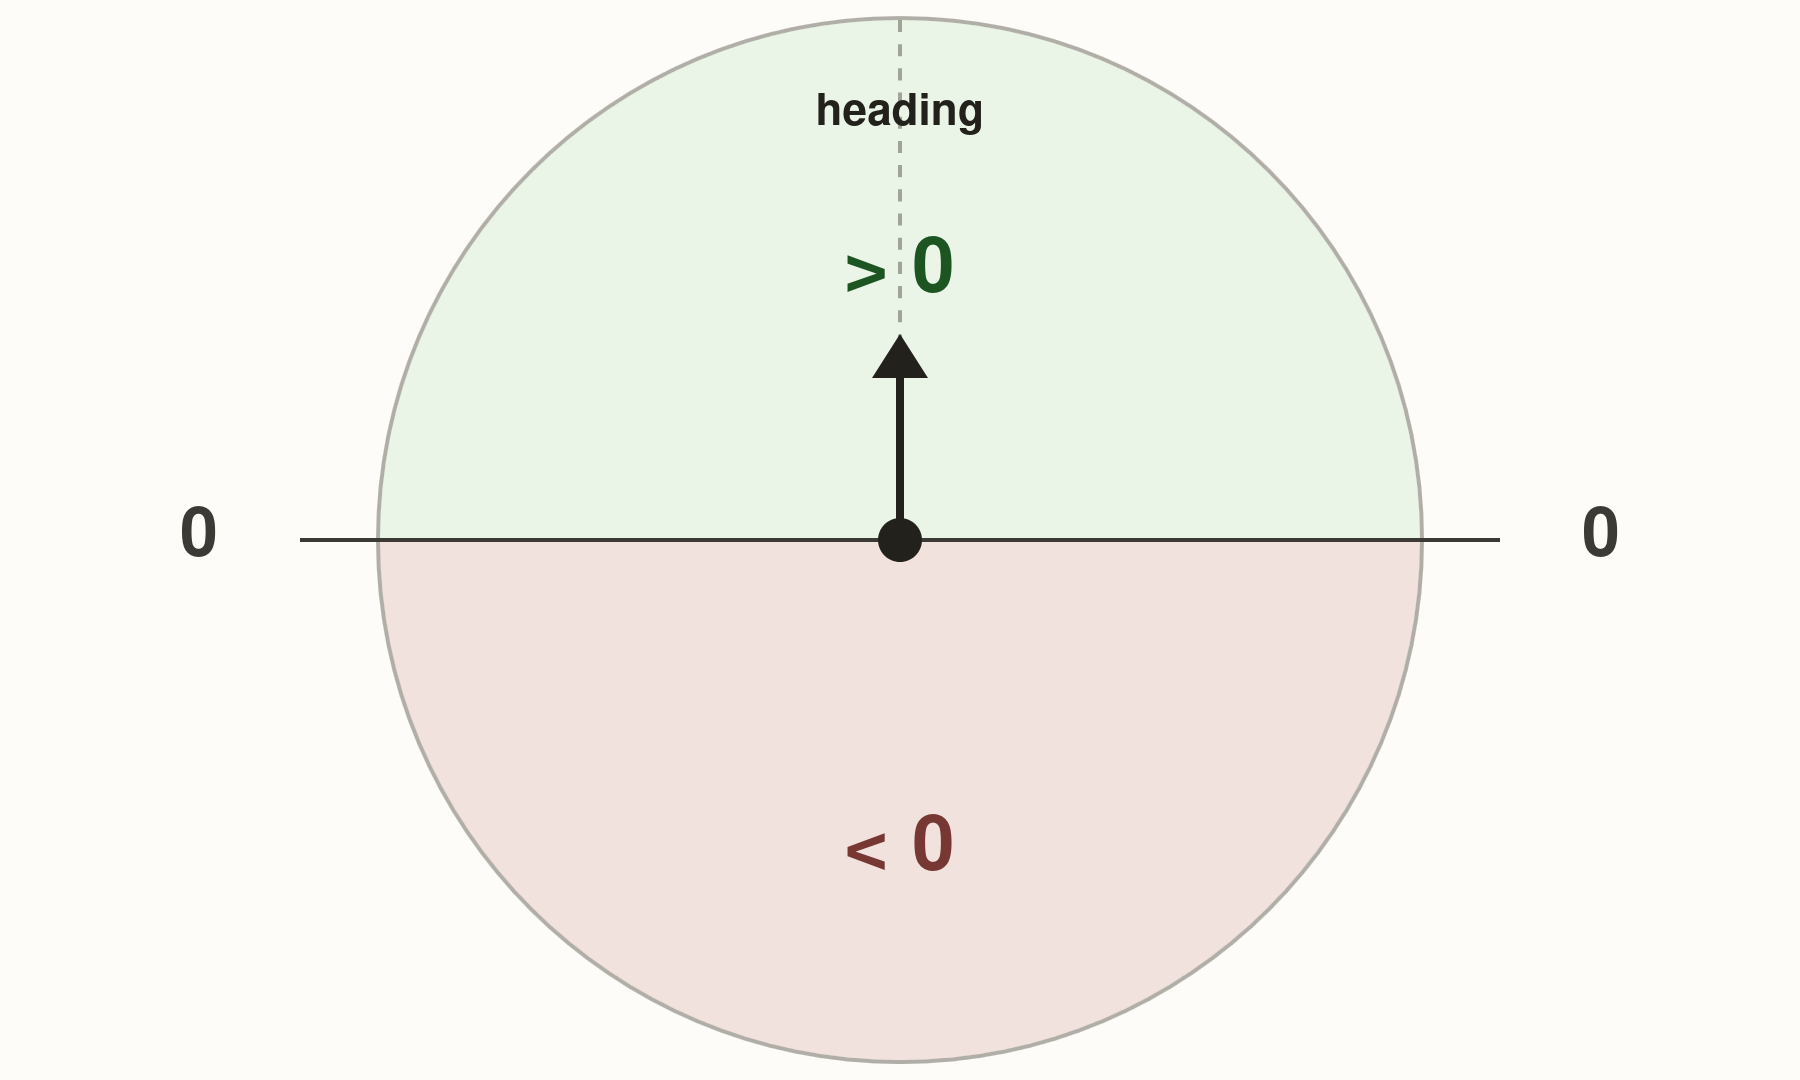
\includegraphics[width=\columnwidth]{Figure_SP.png}
    \caption{Fordward-Backward}
\end{figure}

\subsection{Spatial Classification and Goal Visibility}

The experiment applies the following spatial classification rules:

\begin{align}
    0 \leq s_i \leq 0.707
    &\quad \Rightarrow \quad
    \text{goal beside the robot},
    \\
    s_i > 0.707
    &\quad \Rightarrow \quad
    \text{goal in front of the robot},
    \\
    s_i < 0
    &\quad \Rightarrow \quad
    \text{goal behind the robot}.
\end{align}

The threshold $0.707$ is a design choice corresponding approximately 
to an angular separation of $45^\circ$, since $\cos(45^\circ) \approx 0.707$. 
It separates strongly forward-facing goals from goals that are still 
located in the forward half-plane but are positioned more laterally.

Spatial classification and visibility are related but distinct. 
A goal is considered visible by the selection algorithm only when

\begin{equation}
    s_i \geq 0
\end{equation}

and

\begin{equation}
    d_i > 0.
\end{equation}

The first condition restricts selection to goals in the forward half-plane. The second condition prevents the robot position itself from being selected as a valid goal.

This distinction is important. A goal may be classified as beside the robot because its scalar product is zero, yet still be rejected when its distance is also zero.

\begin{figure}[ht]
    \centering
    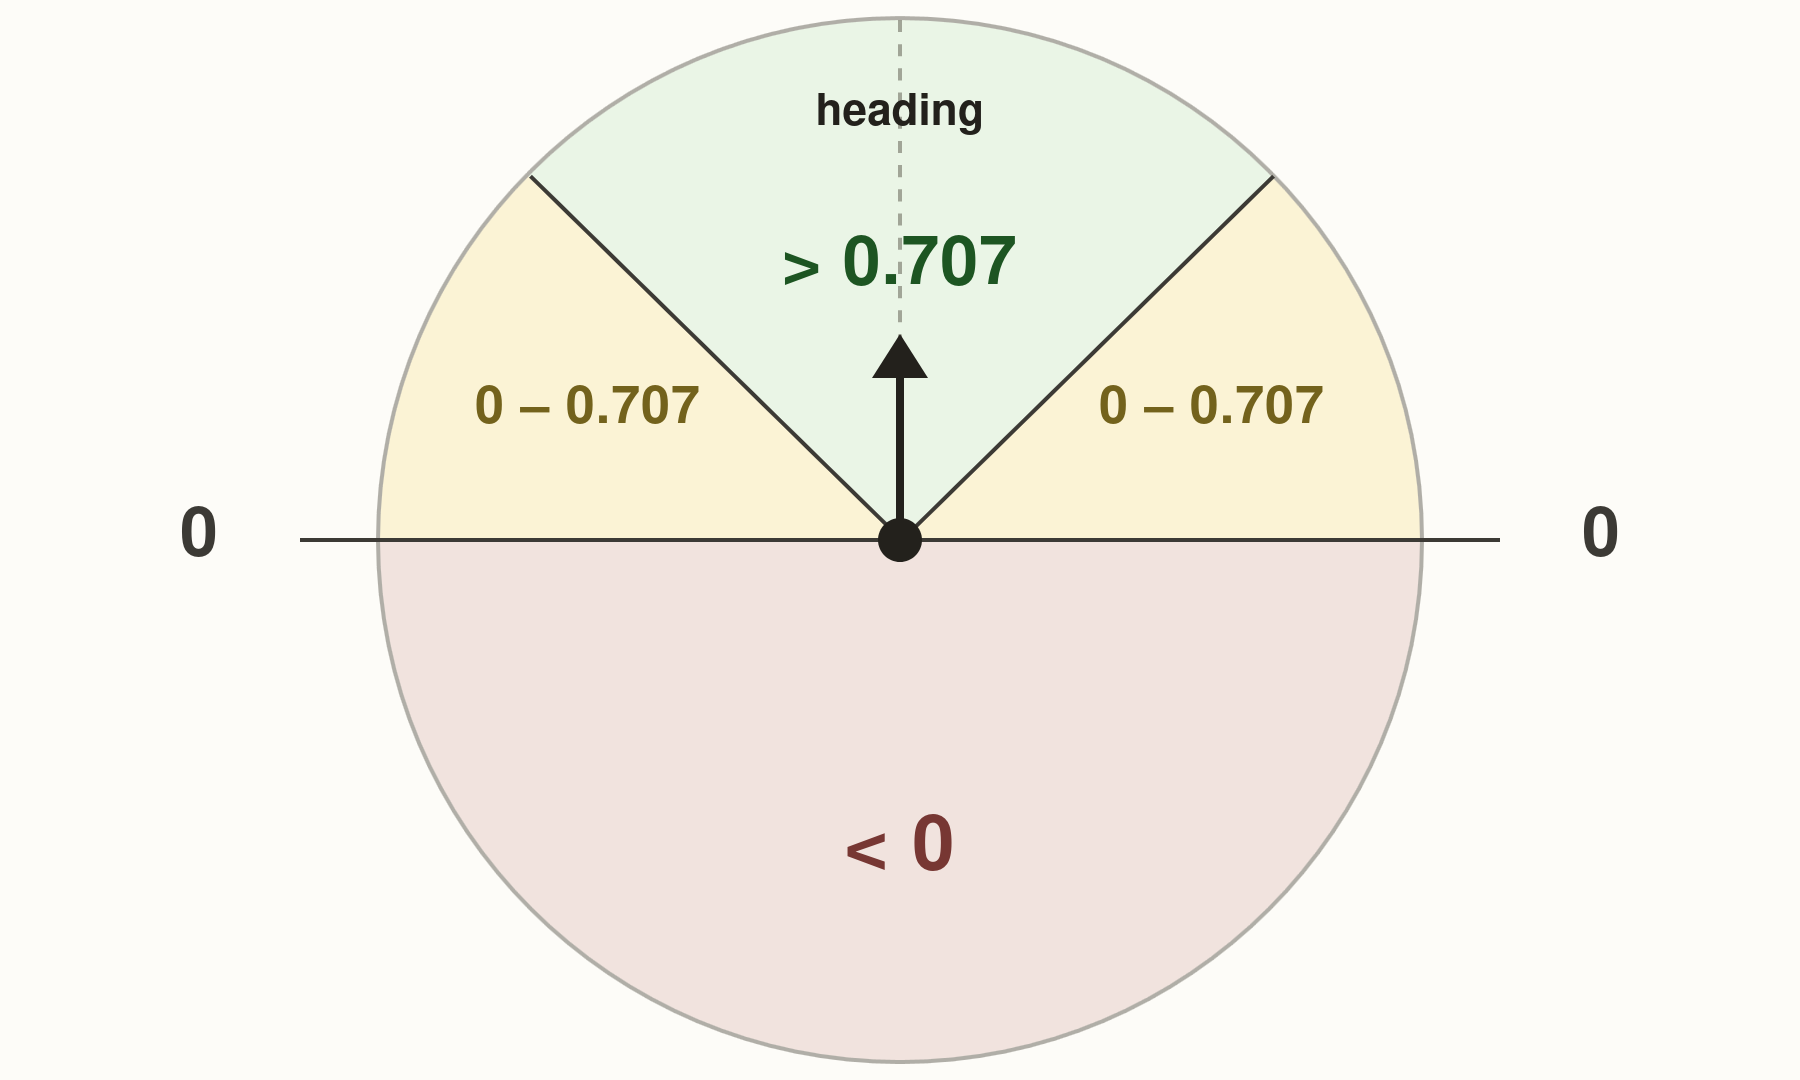
\includegraphics[width=\columnwidth]{Figure_2.png}
    \caption{Fordward-Backward-Beside}
\end{figure}

\section{Project Task}

Define one robot position, a unit heading vector, and several 
candidate goal positions as NumPy arrays. Process all goals iteratively, 
reuse the geometric calculations from Project 1 to obtain each distance 
and normalized goal direction, and calculate the scalar product 
between the robot heading and every goal direction. Classify each goal 
as in front of, beside, or behind the robot, filter the goals using the 
visibility conditions, and select the closest visible goal. Finally, 
print the calculated values, classifications, and selected target.


\begin{thebibliography}{1}

\bibitem{quejido2026vectors}
J. Quejido Barrera,
\textit{Vector-Based Goal Representation for a Mobile Robot},
Road to become more, Project 1, unpublished technical report, 2026.

\end{thebibliography}
% =================================================
\end{document}
% =================================================